\textbf{Chapter 3 Asymptotic Formulas} \\
\thm (Abel's Summation Formula) \\
Let $a\colon\Z^+\to\C$, let $f\colon[1,\infty)\to\C$ be $\mathcal{C}^1$, let $A(x)=\sum_{n\leq x}a(n)$.  Then
\[\sum_{n\leq x}a(n)f(n)=A(x)f(x)-\int_1^xA(t)f'(t)\d t\]

\thm (Euler's Summation Formula) \\
Let $f\colon[1,\infty)\to\C$ be $\mathcal{C}^1$.  Then
\[ \sum_{n\leq x}f(n) = f(1) + \int_1^x f(t)\d t + \int_1^x \chev{t} f'(t)\d t - \chev{x} f(x) \]
where $\chev{x}=x-\floor{x}$. \\
\pf Let $a(n)=1$, $A(x)=\sum_{n\leq x}1=\floor{x}$.  Then by Abel's Summation Formula
\begin{align*}
\sum_{n\leq x}f(n) &= A(x)f(x) - \int_1^x A(t)f'(t) \d t \\
&= \floor{x} f(x) - \int_1^x \floor{t} f'(t) \d t \\
\int_1^x \underbrace{t}_{u} \underbrace{f'(t)\d t}_{\!\d v} &= \brack*{tf(t)-\int f(t)}_1^x \\
&= xf(x) - f(1) - \int_1^x f(t)\d t \\
\therefore \sum_{n\leq x}f(n) &= \floor{x}f(x) - \int_1^x \floor{t} f'(t) \d t %\\
+ \int_1^x t f'(t)\d t - xf(x) + f(1) + \int_1^x f(t) \d t \\
&= f(1) + \int_1^x f(t) \d t + \int_1^x \chev{t} f'(t) \d t - \chev{x} f(x)
\end{align*}
\[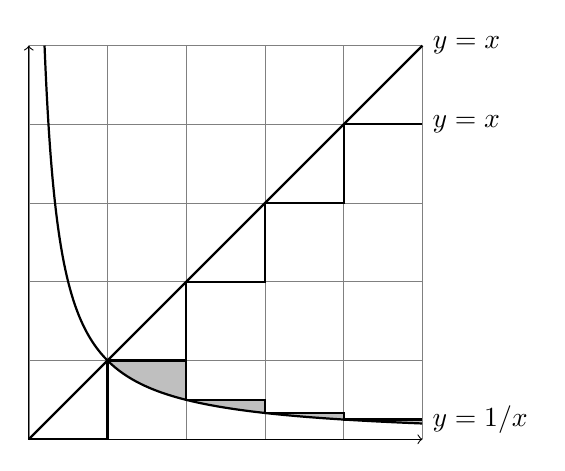
\begin{tikzpicture}[domain=0:5]
\path[fill=lightgray,domain=1:2] plot(\x,1/\x)--(2,1)--cycle;
\path[fill=lightgray,domain=2:3] plot(\x,1/\x)--(3,1/2)--cycle;
\path[fill=lightgray,domain=3:4] plot(\x,1/\x)--(4,1/3)--cycle;
\path[fill=lightgray,domain=4:5] plot(\x,1/\x)--(5,1/4)--cycle;
\draw[gray,very thin](0,0) grid (5,5);
\draw[thick] plot(\x, \x) node[right]{$y=x$};
\draw[thick,samples at={0,...,4,4.999},const plot] plot (\x, {floor(\x)}) node[right]{$y=\floor{x}$};
\draw[thick,samples at={1,...,4,4.999},const plot] plot (\x, {1/floor(\x)}) node[right]{$y=1/\floor{x}$};
\draw[thick,samples at={0.2,0.21,...,5}] plot(\x, 1/\x);
\draw[<->](0,5)--(0,0)--(5,0);
\end{tikzpicture}\]
\eg Euler's constant is
\[ \gamma = \lim_{l\to\infty}\paren[\Big]{\sum_{n=1}^l\frac1n-\ln l} = \lim_{l\to\infty}\paren[\Big]{\int_1^l\frac{1}{\floor{x}}-\frac1x\d x} = \int_1^\infty\frac{x-\floor{x}}{x\floor{x}}\d x \]
\[ \gamma = \int_1^\infty \frac{\chev{t}}{t\floor{t}} \d t \]
Note that the integral does converge since $\frac{\chev{t}}{t\floor{t}}\leq\frac{1}{t(t-1)}$ and $\int_2^\infty\frac{\!\d t}{t(t-1)}=\int_2^\infty\frac{1}{t-1}-\frac{1}{t}\d t=\brack{\ln\frac{t-1}{t}}_2^\infty=-\ln\frac12=\ln2$. \\
\eg How quickly does $\sum_{n=1}^\infty\frac1n-\ln l$ approach $\gamma$?  Find an asymptotic formula for $\sum_{n\leq x}\frac1n$. \\
\soln Use $f(t)=\frac1t$, $f'(t)=-\frac1{t^2}$ in Euler's Summation Formula to get
\begin{align*}
\sum_{n\leq x}\frac1n &= f(1) + \int_1^x f(t)\d t + \int_1^x\chev{t}f'(t)\d t - \chev{x}f(x) \\
&= 1 + \int_1^x\frac1t\d t - \int_1^x\frac{\chev{t}}{t^2}\d t - \frac{\chev{x}}{x} \\
&= 1 + \log x - \int_1^\infty\frac{\chev{t}}{t^2}\d t + \int_x^\infty \frac{\chev{t}}{t^2} \d t + O(\tfrac1x) \\
&= 1 + \log x - c + O(\tfrac1x)\footnote{Aside:
\[ \int_x^\infty\frac{\chev{t}}{t^2}\d t \leq \int_x^\infty\frac1{t^2}\d t = \brack*{-\frac1t}_x^\infty = \frac1x \]} \\
\sum_{n\leq x}\frac1n - \log x &= 1 - c + O(\tfrac1x)
\end{align*}
Take the limit as $x\to\infty$ to get
\[ \gamma = 1-c \qquad (\text{so $\int_1^\infty\frac{\chev{t}}{t^2}\d t=1-\gamma$}) \]
\[ \therefore \sum_{n\leq x}\frac1n = \log x + \gamma + O(\tfrac1x) \]
\eg Find an asymptotic formula for $\sum_{n\leq x}\frac1{n^a}$ where $1<a\in\R$. \\
\soln Use ESF with $f(t)=\frac{1}{t^a}=t^{-a}$, $f'(t)=-at^{-a-1}=\frac{-a}{t^{a+1}}$
\begin{align*}
\sum_{n\leq x}\frac{1}{n^a} &= f(1) + \int_1^x f(t)\d t + \int_1^x\chev{t}f'(t)\d t - \chev{x}f(x) \\
&= 1 + \int_1^x\frac{1}{t^a}\d t - \int_1^x\frac{a\chev{t}}{t^{a+1}}\d t - \frac{\chev{x}}{x^a} \\
&= 1 + \frac{1}{a-1} - \frac{1}{(a-1)x^{a-1}} - \int_1^\infty\frac{a\chev{t}}{t^{a+1}}\d t + \int_x^\infty\frac{a\chev{t}}{t^{a+1}}+O(\tfrac1{x^a})\footnote{Aside:
\[ \int_1^x\frac{1}{t^a} = \int_1^x t^{-a} = \brack*{\frac{t^{-a+1}}{-a+1}}_1^x = \brack*{\frac{-1}{(a-1)t^{a-1}}}_1^x \]} \\
&= \frac{a}{a-1} - \frac{1}{(a-1)x^{a-1}} - c + O(\tfrac{1}{x^a})\footnote{Aside:
\[ \int_x^\infty\frac{a\chev{t}}{t^{a+1}}\d t \leq \int_x^\infty \frac{a}{t^{a+1}}\d t = \brack*{\frac{-1}{t^a}}_x^\infty = \frac{1}{x^a} \]}
\end{align*}
Take the limit as $x\to\infty$
\[ \zeta(a) = \frac{a}{a-1} - c \]
\[ \therefore \sum_{n\leq x}\frac{1}{n^a} = \zeta(a) - \frac{1}{(a-1)x^{a-1}} + O(\tfrac{1}{x^a}) \]
\eg Find an asymptotic formula for
\[ \sum_{n\leq x}\log n = \log\paren[\Big]{\prod_{n\leq x} n} = \log(\floor{x}!) \]
\soln Use ESF with $f(t)=\log t$, $f'(t)=\frac{1}{t}$.
\begin{align*}
\sum_{n\leq x}\log n &= f(1) + \int_1^x f(t)\d t + \int_1^x \chev{t}f'(t)\d t - \chev{x}f(x) \\
&= 0 + \int_1^x \log t \d t + \int_1^x \frac{\chev{t}}{t}\d t - \frac{\chev{x}}{x}\footnote{Aside:$\int_1^x\log t\d t=\brack{t\log t-t}_1^x=x\log x+1$} \\
&= x\log x - x + 1\footnote{Aside: $\int_1^x\frac{\chev{t}}{t}\d t\leq\int_1^x\frac{1}{t}=\log x$} \\
&= x\log x - x + O(\log x)
\end{align*}
\remark If we approximate $\int_1^x\log t$ using a trapezoidal approximation, we can improve this estimate:
\begin{align*}
\sum_{n\leq x}\log n &= x\log x - x + \tfrac12\log x + O(1) \\
&= x\log x - x + \tfrac12\log x + \sqrt{2\pi} + o(1)
\end{align*}
%[diagrams]\\
\begin{center}
\myvcenter{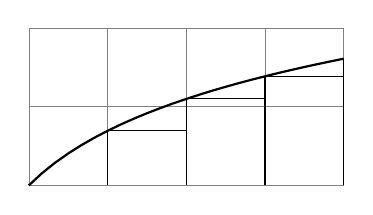
\begin{tikzpicture}[domain=1:5]
\draw[gray,very thin](1,0) grid (5,2);
\draw[thick] plot(\x,{ln(\x)});
\draw (2,0)--(2,{ln(2)})--(3,{ln(2)});
\draw (3,0)--(3,{ln(3)})--(4,{ln(3)});
\draw (4,0)--(4,{ln(4)})--(5,{ln(4)});
\draw (5,{ln(5)})--(5,0);
\end{tikzpicture}} \qquad
\myvcenter{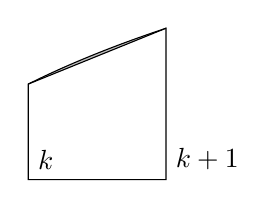
\begin{tikzpicture}[domain=2:3,scale=1.75]
\path[fill=lightgray] plot(\x,{ln(\x)})--(2,{ln(2)});
\draw plot(\x,{ln(\x)});
\draw (2,0)--(2,{ln(2)})--(3,{ln(3)})--(3,0)--cycle;
\node[above right]at(2,0){$k$};
\node[above right]at(3,0){$k+1$};
\end{tikzpicture}}
\end{center}
\eg Find an asymptotic formula for
\[ \sum_{n\leq x}\tau(n) = \sum_{n\leq x}\sum_{d\div n}1 \]
